\documentclass[12pt, a4paper]{article}
\usepackage{enumitem}
\usepackage{float}
\usepackage[left=2cm, right=2cm, top=2cm, bottom=2cm]{geometry}
\usepackage{graphicx}
\usepackage[colorlinks, urlcolor=blue]{hyperref}
\usepackage{minted}
\usepackage{xeCJK}

\renewcommand\arraystretch{1.5}
\setCJKmainfont[AutoFakeBold=1.5]{新細明體}
\setlength{\parindent}{0pt}

\renewcommand\thesubsection{(\arabic{subsection})}

\setminted{
  frame=single,
  tabsize=2,
}

\title{
  \vspace{-1cm}
  Network Administration/System Administration\\
  (NTU CSIE, Spring 2024)\\
  Homework \#12 - Security (Part I)
}
\author{ \Large B12902110 呂承諺}

\begin{document}
  \maketitle

  \section{Cryptography}
  \begin{enumerate}[label=(\alph*)]
    \item \textbf{Steps}
    \begin{enumerate}[label=(\arabic*)]
      \item Download \href{https://drive.google.com/file/d/10iilD7B30Hw6zTYplIenI3CWs5wpIPZM/view?usp=drive_link}{神祕的聲音.wav}.

      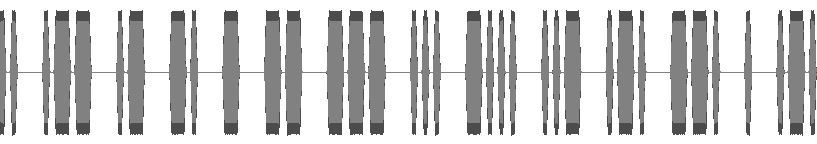
\includegraphics[width=\linewidth]{1-a/1-a_waveform.png}

      \item Inspect the waveform of the audio file, and it looks like Morse code.
      \begin{Verbatim}[frame=single]
.. .-- .- -. - -- --- ... -... ..- .-. --. . .-.
      \end{Verbatim}
      \item Go to \href{https://morsecode.world/international/translator.html}{Morse Code Translator | Morse Code World}
      and paste in the Morse code.
    \end{enumerate}

    \textbf{Flag}\quad\verb|HW12{IWANTMOSBURGER}|

    \pagebreak
    \item \textbf{Steps}
    \begin{enumerate}[label=(\arabic*)]
      \item Download \href{https://drive.google.com/file/d/1HP6nANS-149jWhmyjAIOeEt4jSnxb3br/view?usp=drive_link}{門上的密文.txt}.
      \begin{Verbatim}[frame=single, commandchars=\\\{\}]
uj12{zbf_ohetre_vf_gur_orfg}
      \end{Verbatim}
      \item According the problem's hint and the chiphertext's format, it looks like a
      Caesar cipher. Therefore, code a simple C++ program to try out all the possible rotations.
      \inputminted[fontsize=\small]{cpp}{1-b/caesar_cipher.cpp}
      \item Compile and run our program. We obtain the flag with rotation 13.
      \begin{Verbatim}[frame=single]
$ g++ -o caesar_cipher caesar_cipher.cpp
$ ./caesar_cipher < 門上的密文.txt
rotate 0: uj12{zbf_ohetre_vf_gur_orfg}
rotate 1: vk12{acg_pifusf_wg_hvs_psgh}
...
rotate 13: hw12{mos_burger_is_the_best}
...
      \end{Verbatim}
    \end{enumerate}

    \textbf{Flag}\quad\verb|hw12{mos_burger_is_the_best}|

    \textbf{References}
    \begin{itemize}
      \item \href{https://en.wikipedia.org/wiki/Caesar_cipher}{Caesar cipher - Wikipedia}
    \end{itemize}

    \pagebreak
    \item \textbf{Steps}
    \begin{enumerate}
      \item Download \href{https://drive.google.com/file/d/1KB4m0cUQopZ0h09-Nr7RwOD2-HhccwVf/view?usp=drive_link}{blaise的紙條.txt}.
      \begin{Verbatim}[frame=single, fontsize=\scriptsize, breaklines]
Xolffp, O'zv nswo wigzzzu kpgv SSJ NIJHYI, gru U bguctk cfg kson juqv YCK COIMII fcg. Jz zz'w eah lpi dagy ffgvvck, afgzv zil hi rnzw ui gogb gd kpgv uj ktsas xvrmtucmt vlxkvdg xpl dk? M kdiku sfav kmglf, mf livx tjfy ku gyackf qyogyqjws zcgzfdg qpo knmew W'v mcbk.

Pfayaoa wuvnmfv ui tgxttwfh og gru qbbpsztk r sfwbn dkec fcyfnykv jacf. Myk si bzco jz Z iee ffwbn puy ka ggnyknmes wf sykave!
TK12{tmuzyi_nmblt_GFY_FLDUWS_nfu}

MOSBURGER
      \end{Verbatim}
      \item According to the hints, this piece of text may be encrypted in Vigenère cipher
      with MOSBURGER as the key. Code a simple C++ program to decrypt the text.
      \inputminted[fontsize=\small]{cpp}{1-c/vigenere_cipher.cpp}
      \item Compile and run our program. The flag is in the output.
      \begin{Verbatim}[frame=single, fontsize=\small, breaklines]
$ g++ -o vigenere_cipher vigenere_cipher.cpp
$ ./vigenere_cipher < blaise的紙條.txt
Lately, I've been craving some MOS BURGER, and I notice you want some MOS BURGER too.
...
HW12{blaise_wants_MOS_BURGER_too}
      \end{Verbatim}
    \end{enumerate}

    \textbf{Flag}\quad\verb|HW12{blaise_wants_MOS_BURGER_too}|

    \textbf{References}
    \begin{itemize}
      \item \href{https://en.wikipedia.org/wiki/Vigen%C3%A8re_cipher}{Vigenère cipher - Wikipedia}
    \end{itemize}

    \pagebreak
    \item \textbf{Steps}
    \begin{enumerate}[label=(\arabic*)]
      \item Download \href{https://drive.google.com/file/d/1XcwAgPA3HW6MzDrwJdStTmXGwMelPqFg/view?usp=drive_link}{小福門口的告示.txt}.
      \begin{Verbatim}[frame=single, fontsize=\scriptsize, breaklines]
Jgmh Dmovgj Wvsqzaghs,

F lzkg qlfs agssmtg rfxjs yzv ugoo. F ma uhfqfxt qz mjjhgss mx vxrzhqvxmqg fxwfjgxq qlmq zwwvhhgj mq zvh AZS NVHTGH ozwmqfzx hgwgxqoy. Fq lms wzag qz zvh mqqgxqfzx qlmq qlg rhzxq jzzh zr zvh hgsqmvhmxq ums nhzigx, hgsvoqfxt fx fxwzxdgxfgxwg qz amxy zr yzv, zvh ozymo wvsqzaghs. Kogmsg mwwgkq ay sfxwghgsq mkzoztfgs rzh mxy jfshvkqfzx qlfs amy lmdg wmvsgj.

...

Umha hgtmhjs,
mhwlgh wlgx
Amxmtgh, AZS NVHTGH
      \end{Verbatim}
      \item Observe the text, and we discover that ``AZS NVHTGH" is repeated many times. We
      suspect that it maps to ``MOS BURGER".

      So, we code a simple C++ program that handles character substitution. We
      will update the mapping gradually as we guess out more and more characters.
      \begin{minted}[fontsize=\small]{cpp}
#include <iostream>

int main() {
  // Gradually updated.
  const char kMap[27] = "MBCDEFERIJKLMBOPQRSGUUWXYO";

  std::string s;
  while (std::getline(std::cin, s)) {
    for (char& c : s) {
      if (!isalpha(c)) {
        continue;
      }
      char base;
      if (islower(c)) {
        base = 'a';
      } else {
        base = 'A';
      }
      c = base + kMap[c - base] - 'A';
    }
    std::cout << s << std::endl;
  }
  return 0;
}
      \end{minted}

      \item The decrypted for now looks something like this.
      \begin{Verbatim}[frame=single, fontsize=\scriptsize, breaklines]
Jemr Dmouej Wusqomers,

F loke qlfs messmge rfxjs you ueoo. F mm urfqfxg qo mjjress mx uxrorquxmqe fxwfjexq qlmq owwurrej mq our MOS BURGER oowmqfox rewexqoy. Fq lms wome qo our mqqexqfox qlmq qle rroxq joor or our resqmurmxq ums broiex, resuoqfxg fx fxwoxdexfexwe qo mmxy or you, our ooymo wusqomers. Koemse mwwekq my sfxweresq mkooogfes ror mxy jfsrukqfox qlfs mmy lmde wmusej.
...
LU12{qle_broiex_rroxq_joor_or_MOS}
...
Umrm regmrjs,
mrwler wlex
Mmxmger, MOS BURGER
      \end{Verbatim}
      Referring back to the original message, we suspect the following mappings.

      \begin{tabular}{|cc|}
        \hline \textbf{Chipertext} & \textbf{Plaintext} \\\hline
        Jgmh & Dear \\
        Wvsqzaghs & Customers \\
        agssmtg & message \\
        LU & HW \\
        Umha hgtmhjs & Warm regards \\\hline
      \end{tabular}

      \vspace{0.5\baselineskip}
      \item Decrypt the ciphertext with the updated mapping. Now it looks something
      like this.
      \begin{Verbatim}[frame=single, fontsize=\scriptsize, breaklines]
...

As a gesture or goodwfoo, we'd ofie to orrer a 10% dfscouxt ox your xeet meao wfth us. ...

Thaxi you oxce agafx ror your uxderstaxdfxg, axd we oooi rorward to weocomfxg you baci to a ruooy okeratfoxao axd fmkroded MOS BURGER eekerfexce dery soox.
      \end{Verbatim}
      The last two paragraphs actually give us quite a lot of information.

      \begin{tabular}{|cc|}
        \hline \textbf{Chipertext} & \textbf{Plaintext} \\\hline
        orrer & offer \\
        dfscouxt & discount \\
        xgeq & next \\
        Qlmxi & Thank \\
        yzv & you \\\hline
      \end{tabular}\quad
      \begin{tabular}{|cc|}
        \hline \textbf{Chipertext} & \textbf{Plaintext} \\\hline
        zxwg & once \\
        mtmfx & again \\
        rzh & for \\
        vxjghsqmxjfxt & understanding \\
        ugowzafxt & welcoming \\\hline
      \end{tabular}

      \vspace{0.5\baselineskip}
      \item Now the message is almost cracked.
      \begin{Verbatim}[frame=single, fontsize=\scriptsize, breaklines]
Dear Dalued Customers,

... Klease accekt my sincerest akologies for any disruktion this may hade caused.

...

We recognipe that this issue has been disakkointing

...

To address this issue kromktly, we'de arranged for a krofessional rekair. ... If you hade any concerns, cuestions, or feedback, klease feel free to reach out to me directly or skeak with any member of our team.
      \end{Verbatim}

      \begin{tabular}{|cc|}
        \hline \textbf{Chipertext} & \textbf{Plaintext} \\\hline
        hgwztxfpg & recognize \\\
        Kogmsg & Please \\
        mwwgkq & accept \\\hline
      \end{tabular}\quad
      \begin{tabular}{|cc|}
        \hline \textbf{Chipertext} & \textbf{Plaintext} \\\hline
        cvgsqfzxs & questions \\
        ug'dg & we've \\\hline
      \end{tabular}

      \vspace{0.5\baselineskip}
      \item Now we have figured out the mapping. ``ABC...XYZ" maps to
      ``MBQVXIERKDPHABLZTFSGWUCNYO". We use this to crack the flag.
    \end{enumerate}
    \textbf{Flag}\quad\verb|HW12{the_broken_front_door_of_MOS}|

    \pagebreak
    \item \textbf{Steps}
    \begin{enumerate}[label=(\arabic*)]
      \item Download \verb|english-menu_A.png| and \verb|english-menu_B.png|. We
      discover that they have the exact same resolution, so it make come down to
      some kind of filtering.

      Furthermore, the two images only contain black and white pixels. We suspect
      that the two images can be merged pixel by pixel with bitwise XOR.

      \item Code a simple Python script that performs pixel-wise XOR
      with Pillow and numpy.
      \inputminted[fontsize=\small]{python}{1-e/xor_image.py}
    \end{enumerate}

    \textbf{Result}\quad The resulting image indeed contains the flag.

    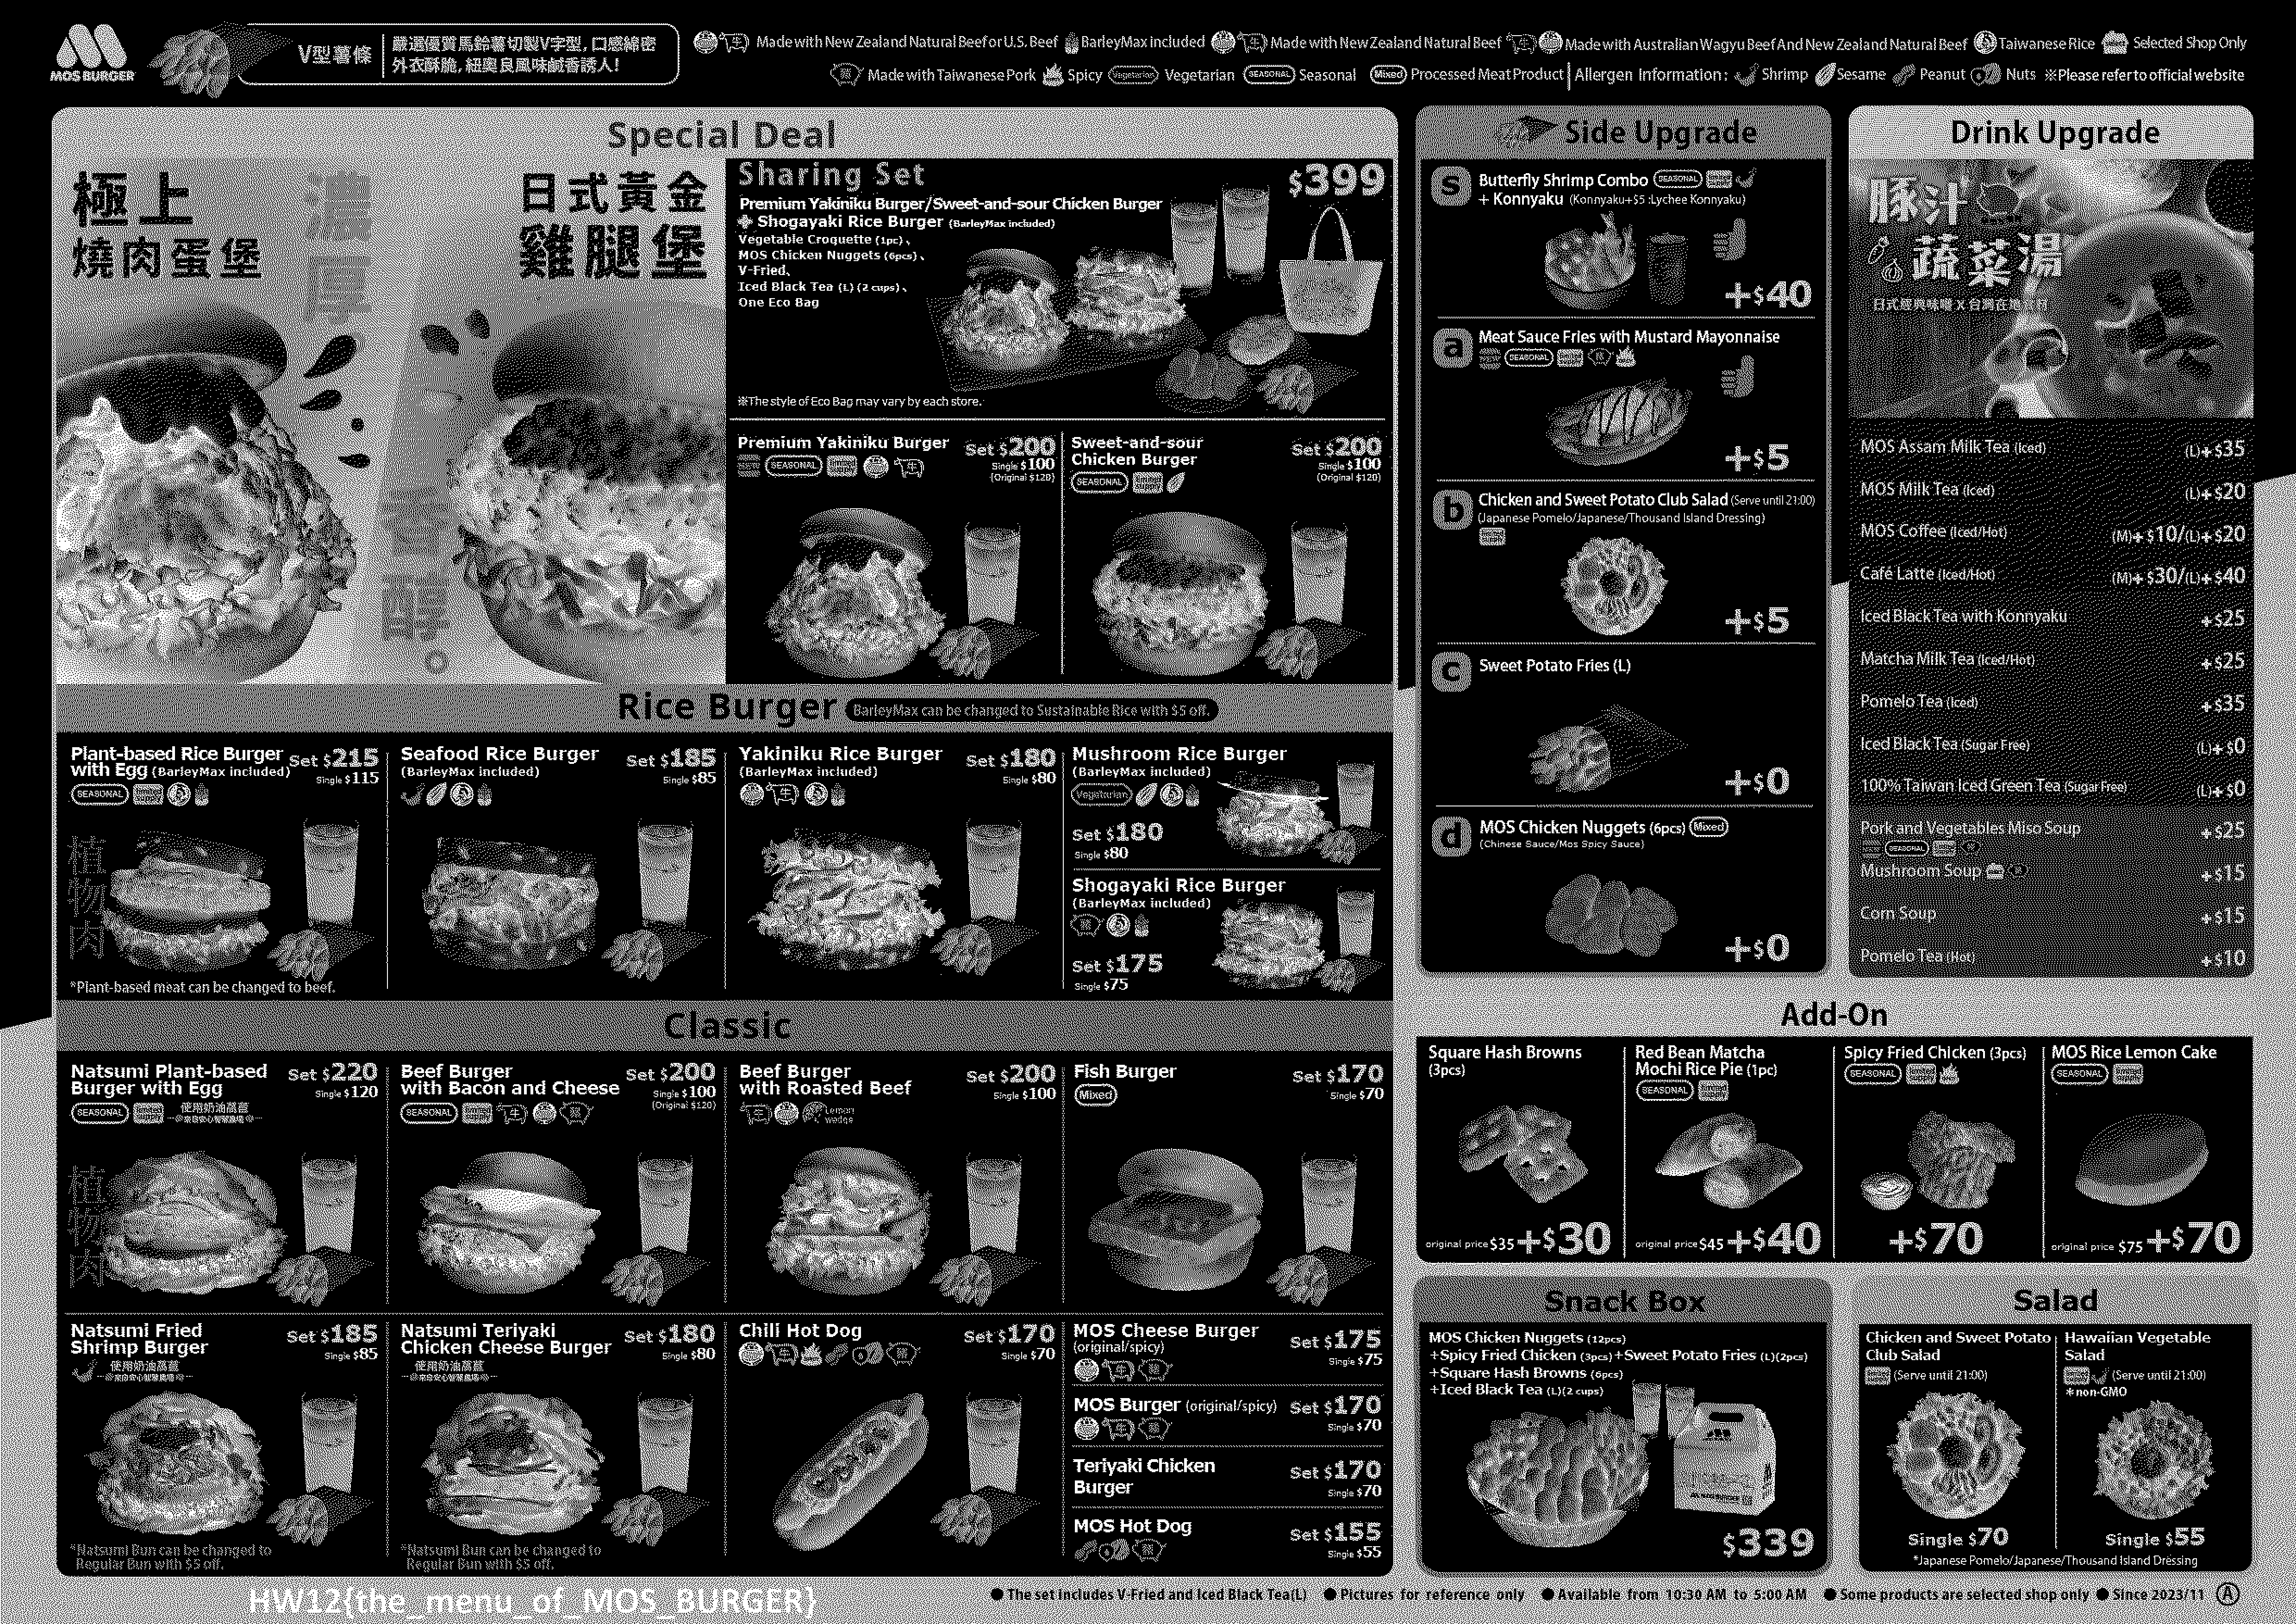
\includegraphics[width=0.7\linewidth]{1-e/xor.png}

    \vspace{0.5\baselineskip}
    \textbf{Flag}\quad\verb|HW12{the_menu_of_MOS_BURGER}|

    \vspace{0.5\baselineskip}
    \textbf{References}
    \begin{itemize}
      \item \href{https://pillow.readthedocs.io/en/stable/reference/Image.html}{Image Module - Pillow (PIL Fork) 10.3.0 documentation}
    \end{itemize}
  \end{enumerate}

  \pagebreak
  \section{DNS security}
  \begin{enumerate}[label=(\alph*)]
    \item \textbf{DNS Spoofing} is a general term that refers to any attempt
    to hijack the DNS service and send out malicious DNS records to clients.
    If DNS services are compromised, incorrect IP addresses for domains
    could flow around the Internet, and network traffic could be directed to
    unintended places. This could cause other services to become inaccessible,
    or even expose data to attackers.
    \item \textbf{DNSSEC} allows DNS records to be signed with public key
    cryptography, providing a method to authenticate responses returned from
    servers. A chain of trust is built from the root server down to the
    authoritative server. If an attacker is trying to spoof DNS records,
    it would not have the legitimate signature, and the recursive resolver
    or client can simply reject the response.
    \item \textbf{DNS Cache Poisoning} refers to an attempt to insert
    malicious records into the DNS cache of a client or DNS resolver.
    This would cause future queries to return the attacker-determined
    location, and network traffic could be directed unwanted locations.
    \item An \textbf{NXDOMAIN attack} is a type of denial-of-servuce attack, where
    the attacker floods a DNS server with queries that ask for nonexistent domains.
    This could  overload the server or fill up the server's cache, and the service
    may go down.
    \item The following measures could help prevent DNS attacks:
    \begin{itemize}
      \item Opt for secure DNS protocols, such as DNSSEC, DNS over HTTPS,
      or DNS over TLS, to prevent DNS spoofing attacks.
      \item Deploy multiple redundant DNS servers with load balancing to prevent
      DDoS attacks.
      \item Limit the rate at which queries could be made.
      \item Restrict the hosts that can access our DNS service. For example,
      in a school or company, we only need to provide service to clients
      inside it.
    \end{itemize}

    The following measures could help detect DNS attacks:
    \begin{itemize}
      \item If an abnormally large amount of queries are coming from similar
      sources, this may be a DDoS attack.
      \item If an abnormally large amount of response are coming from similar
      sources, this may be a DNS spoofing attack.
    \end{itemize}
  \end{enumerate}

  \textbf{References}
  \begin{itemize}
    \item \href{https://en.wikipedia.org/wiki/DNS_spoofing}{DNS spoofing - Wikipedia}
    \item \href{https://en.wikipedia.org/wiki/Domain_Name_System_Security_Extensions}{Domain Name System Security Extensions - Wikipedia}
    \item \href{https://www.cloudflare.com/learning/dns/dns-cache-poisoning/}{What is DNS cache poisoning? | DNS spoofing | Cloudflare}
    \item \href{https://www.cloudflare.com/learning/dns/dns-security/}{What is DNS Security? | DNSSEC | Cloudflare}
    \item \href{https://security.stackexchange.com/questions/33257/dns-spoofing-vs-dns-cache-poisoning}{DNS Spoofing vs DNS Cache Poisoning - Information Security Stack Exchange}
  \end{itemize}

  \pagebreak
  \section{CIA Triad \& Threat Modeling}
  \begin{enumerate}[label=(\alph*)]
    \item
    \begin{enumerate}[label=(\arabic*)]
      \item Taiwan's household registration database leaks to the dark web.

      Confidentiality: Sensitive information isn't kept privately enough.

      Availability: According to my previous experiences, the average government
      employee has too much access to citizens' personal information. All they need is
      enter your ID number.

      \item NTU Office of Academic Affairs' website is hacked by Chinese attackers.

      Confidentiality: There are security weaknesses in our system
      for those attackers across the Taiwan Strait to exploit.

      Integrity: The web pages are maliciously modified by the attackers.
    \end{enumerate}
    \item \textbf{Assumptions}
    \begin{itemize}
      \item A password is required to login to any account. There is no guest account.
    \end{itemize}

    \textbf{Threat models and countermeasures}
    \begin{itemize}
      \item \textbf{Threat model}: Someone sneakily access the computer when the owner leaves
      it without locking the account.

      \textbf{Countermeasure}: Lock the account immediately whenever the owner is not using
      the computer.

      \item \textbf{Threat model}: Someone boots into the computer with a USB installation media,
      mounts your filesystem, and access your data.
      Or even they find a way to extract \verb|/etc/shadow| from the filesystem and crack your password.

      \textbf{Countermeasure}: Encrypt the root filesystem, and use strong login passwords.
    \end{itemize}

    \item

    \item \textbf{Assumptions}
    \begin{itemize}
      \item Members of different groups wouldn't see nor hear each other physically.
    \end{itemize}

    \textbf{Threat models and countermeasures}
    \begin{itemize}
      \item \textbf{Threat model}: Members of different groups use online
      live chat services to communicate with each other.

      \textbf{Countermeasure}: During the exam, setup firewall rules across
      the classroom to deny access to popular online chat services.

      \item \textbf{Threat model}: Members of different groups exchange data
      with services that would be unreasonable for us to ban for the purpose
      of the exam, such as GitHub or Pastebin.

      \textbf{Countermeasure}: Demand that students record or broadcast their
      screens during the exam. The screen recordings could be the TAs' reference
      for checking whether cheating is involved.
    \end{itemize}
  \end{enumerate}

  \pagebreak
  \section{Web Security}
  \subsection{OWASP Juice Shop}
  \begin{enumerate}[label=(\alph*)]
    \item \textbf{DOM XSS}

    \textbf{Steps}

    Search for \mintinline{html}{<iframe src="javascript:alert(`xss`)">} in
    the search box in the navbar.

    \textbf{Result}

    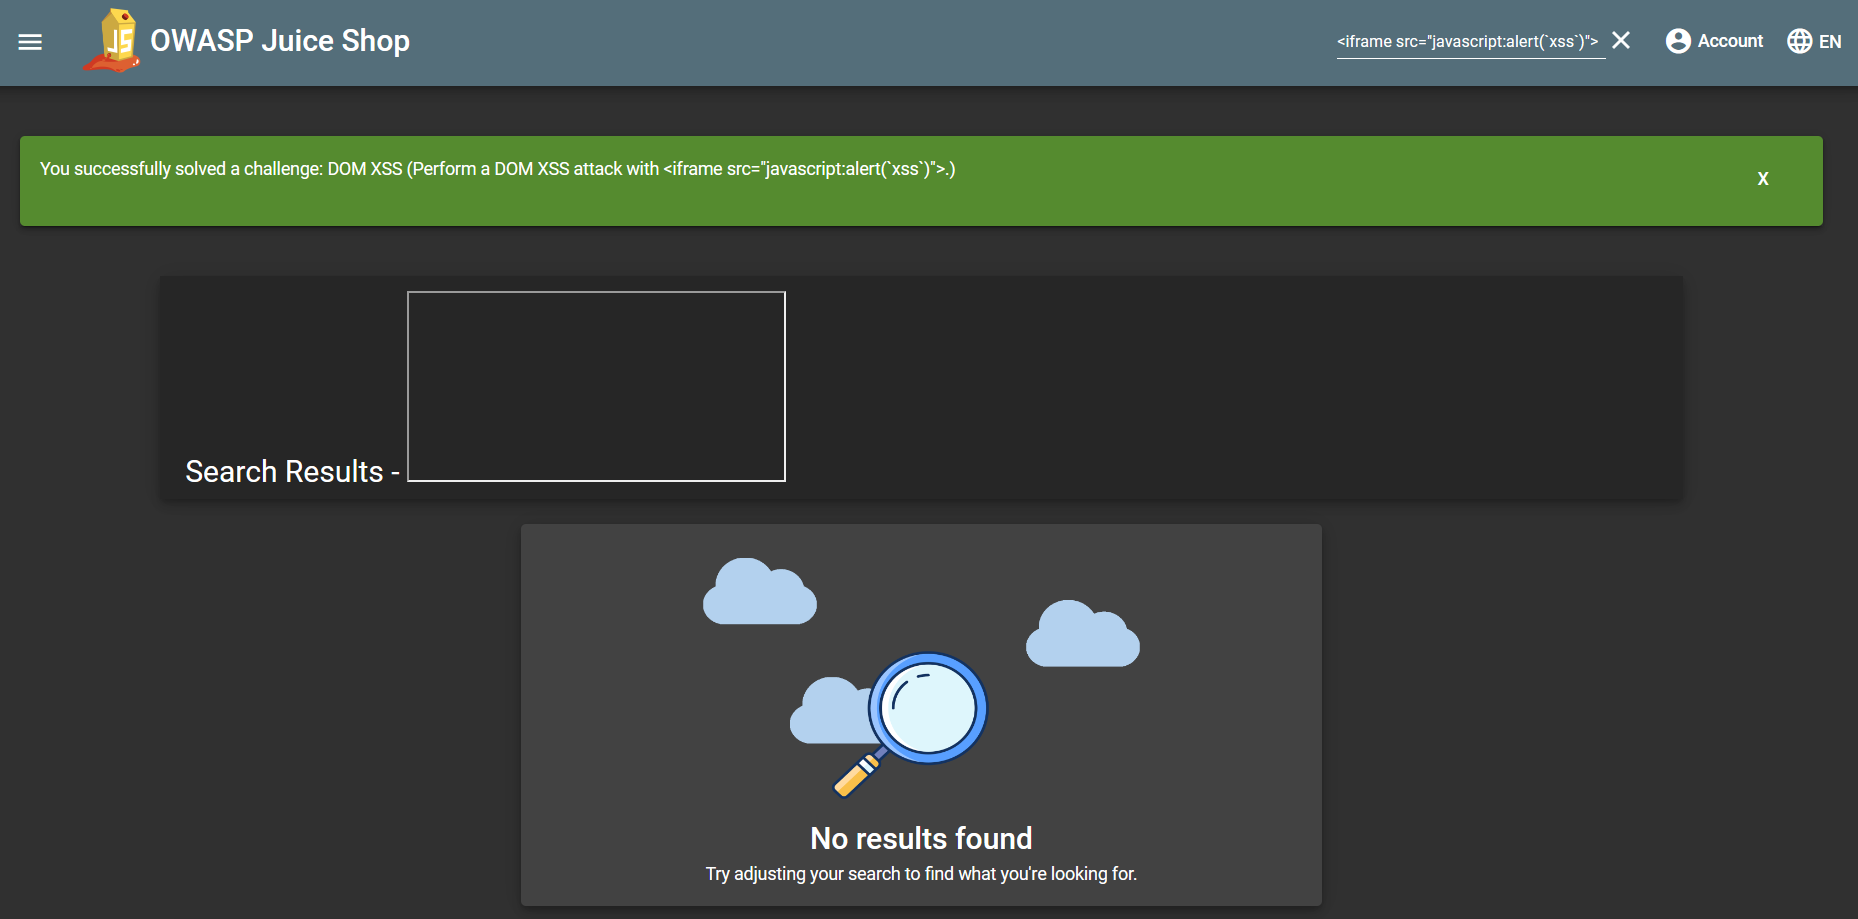
\includegraphics[width=\linewidth]{4-1-a.png}

    \textbf{Explanation}

    This attack is a type of XSS attack, where malicious code is injected
    into the website. In this example, the search query is inserted into
    the HTML DOM, so we can forge the search query to contain HTML elements.

    To prevent this type of attack, we can escape characters that are related
    to HTML tags.

    \textbf{References}
    \begin{itemize}
      \item \href{https://en.wikipedia.org/wiki/Cross-site_scripting}{Cross-site scripting - Wikipedia}
      \item \href{https://pwning.owasp-juice.shop/companion-guide/latest/part2/xss.html}{Cross Site Scripting (XSS) :: Pwning OWASP Juice Shop}
    \end{itemize}

    \pagebreak
    \item \textbf{Bonus Payload}

    \textbf{Steps}

    Search for \mintinline[breaklines, breakanywhere, breakanywheresymbolpre=]{html}{<iframe width="100%" height="166" scrolling="no" frameborder="no" allow="autoplay" src="https://w.soundcloud.com/player/?url=https%3A//api.soundcloud.com/tracks/771984076&color=%23ff5500&auto_play=true&hide_related=false&show_comments=true&show_user=true&show_reposts=false&show_teaser=true"></iframe>} in
    the search box in the navbar.

    \textbf{Result}

    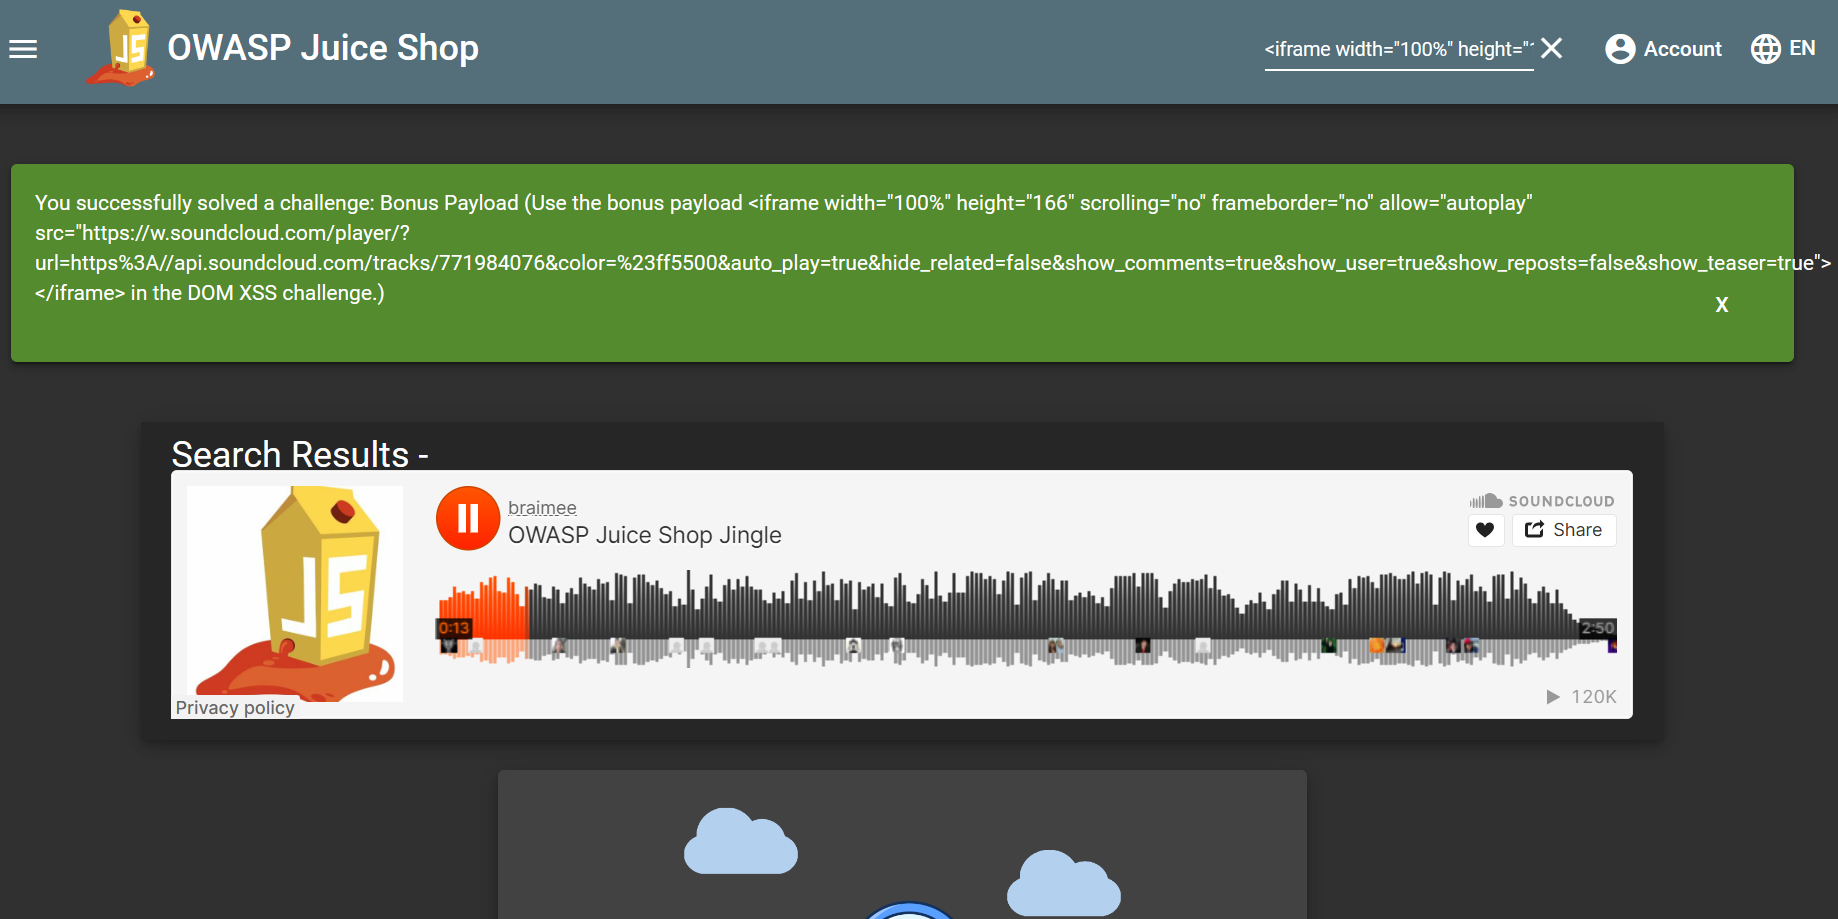
\includegraphics[width=\linewidth]{4-1-b.png}

    \textbf{Explanation}\quad Same as (a).

    \pagebreak
    \item \textbf{Confidential Document}

    \textbf{Steps}
    \begin{enumerate}[label=(\roman*)]
      \item In the ``About Us" (\verb|/#/about|) page, there is a hyperlink to
      \verb|/ftp/leagl.md|.

      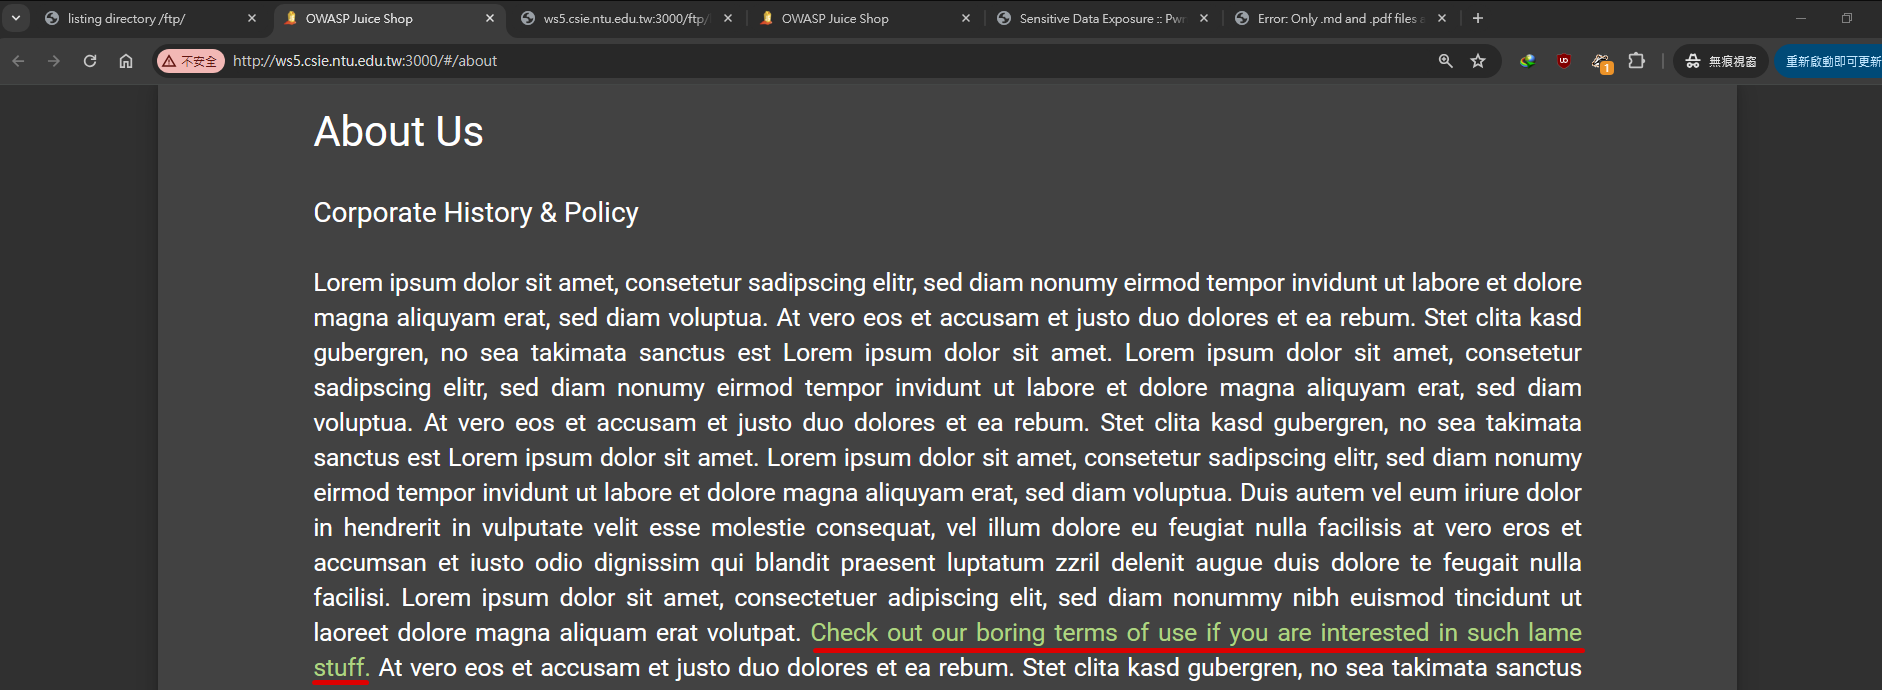
\includegraphics[width=\linewidth]{4-1-c_about.png}

      \item Access \verb|/ftp/|, and a web page with directoy listings shows up.

      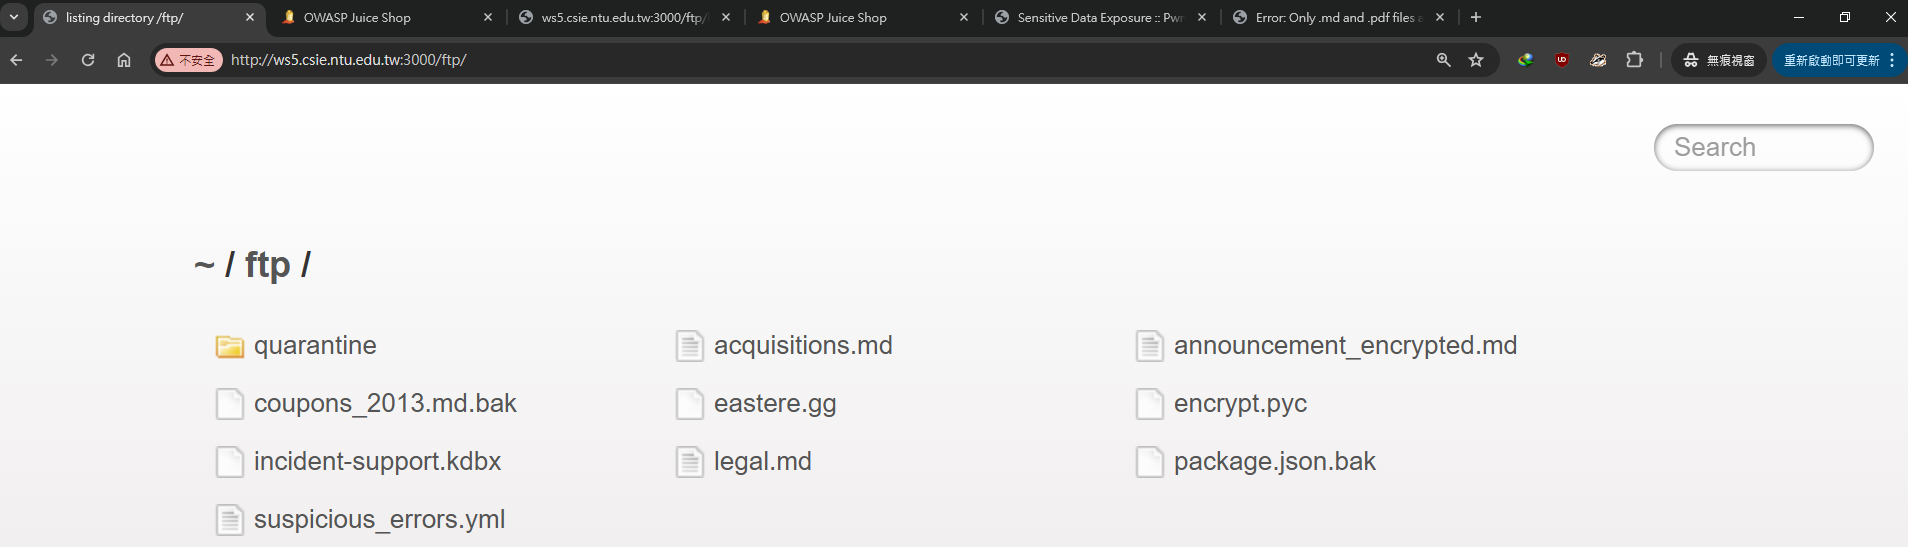
\includegraphics[width=\linewidth]{4-1-c_ftp.png}

      \item Access \verb|/ftp/acquisitions.md|, and the challenge is solved.

      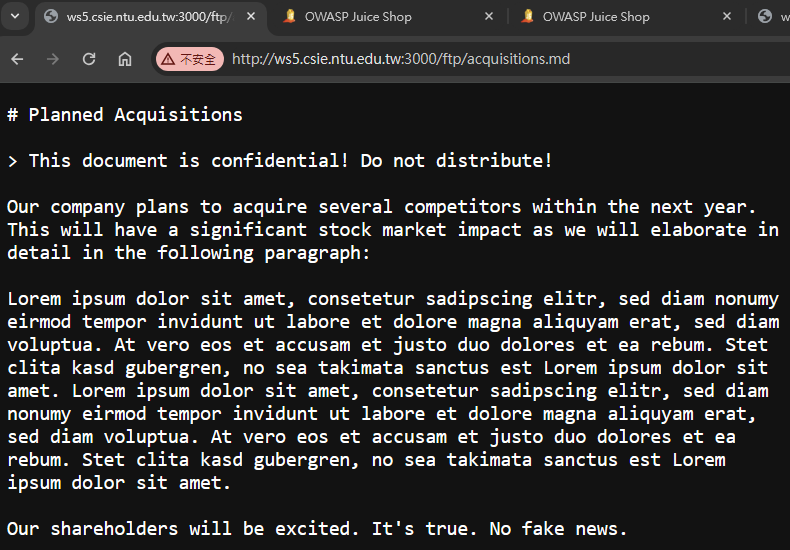
\includegraphics[width=0.8\linewidth]{4-1-c_acquisitions.png}
    \end{enumerate}

    \pagebreak
    \textbf{Result}

    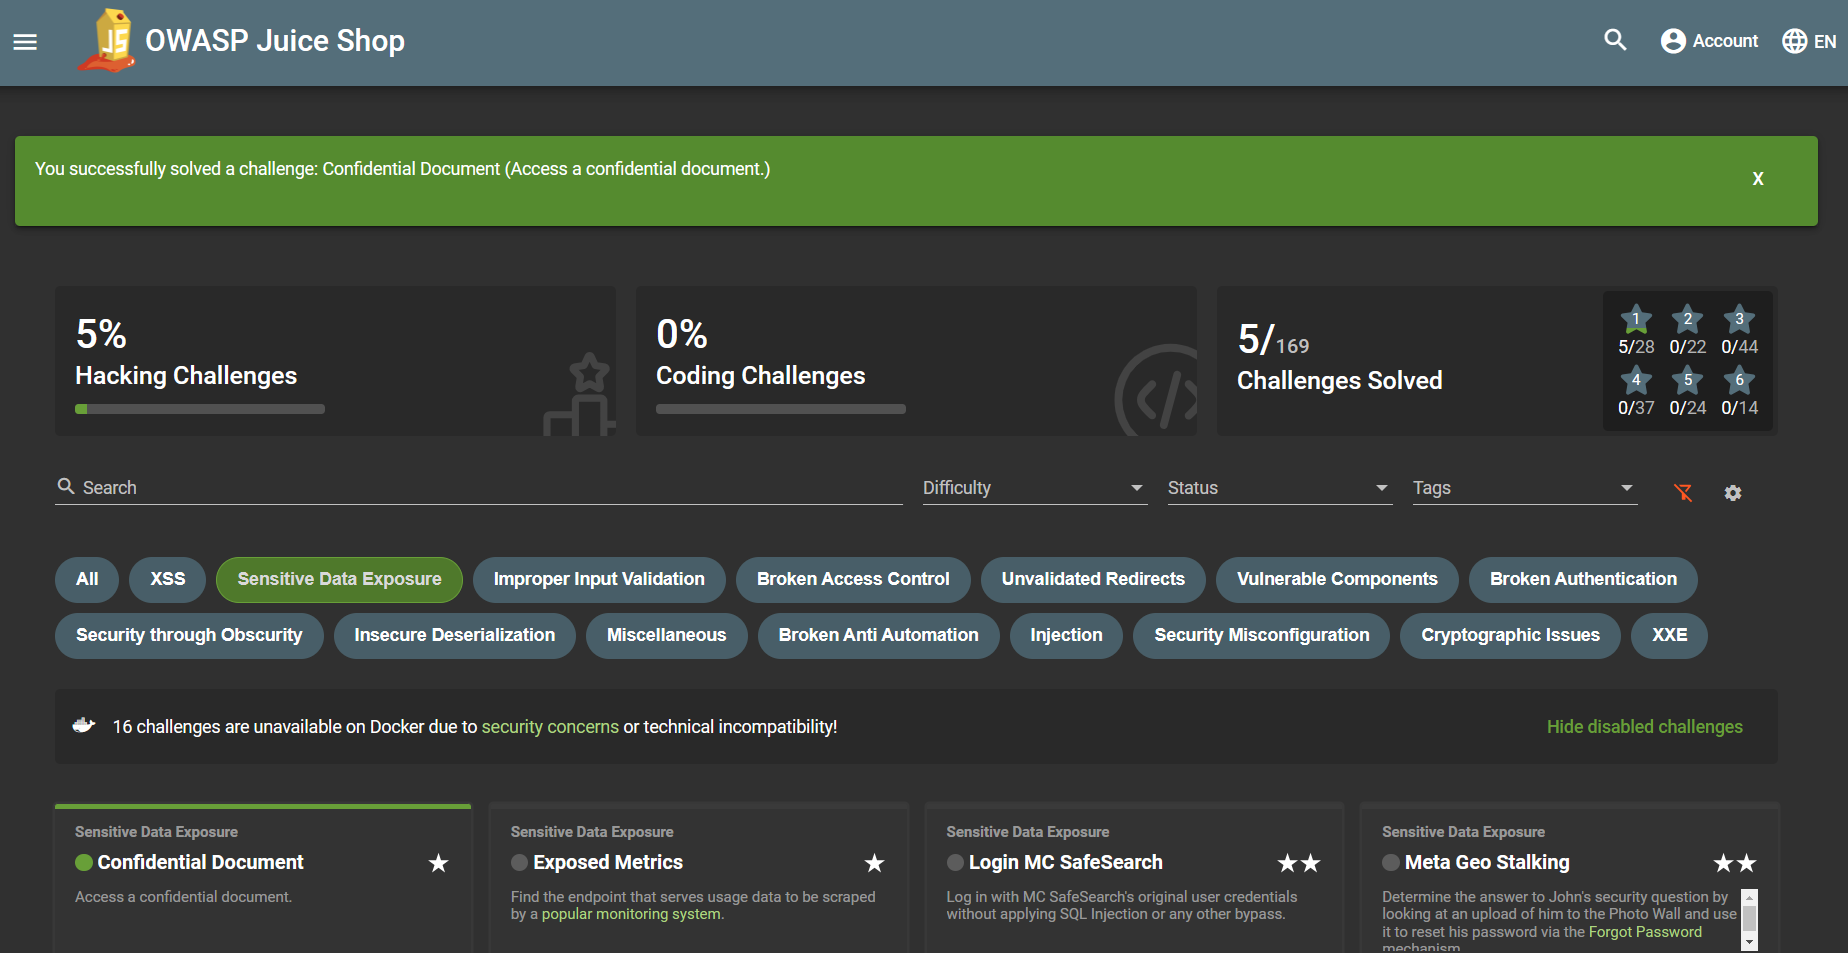
\includegraphics[width=\linewidth]{4-1-c_solved.png}

    \textbf{Explanation}

    This attack is possible because a web page containing a directory listing
    is exposed to the public.

    To prevent this type of attack, we deny directory listing web pages
    from being accessed publicly, and minimize the static files being
    served.

    \pagebreak
    \item \textbf{Error Handling}

    \textbf{Steps}

    From the directory listing (\verb|/ftp/|), access \verb|encrypt.pyc|. An
    error page appears.

    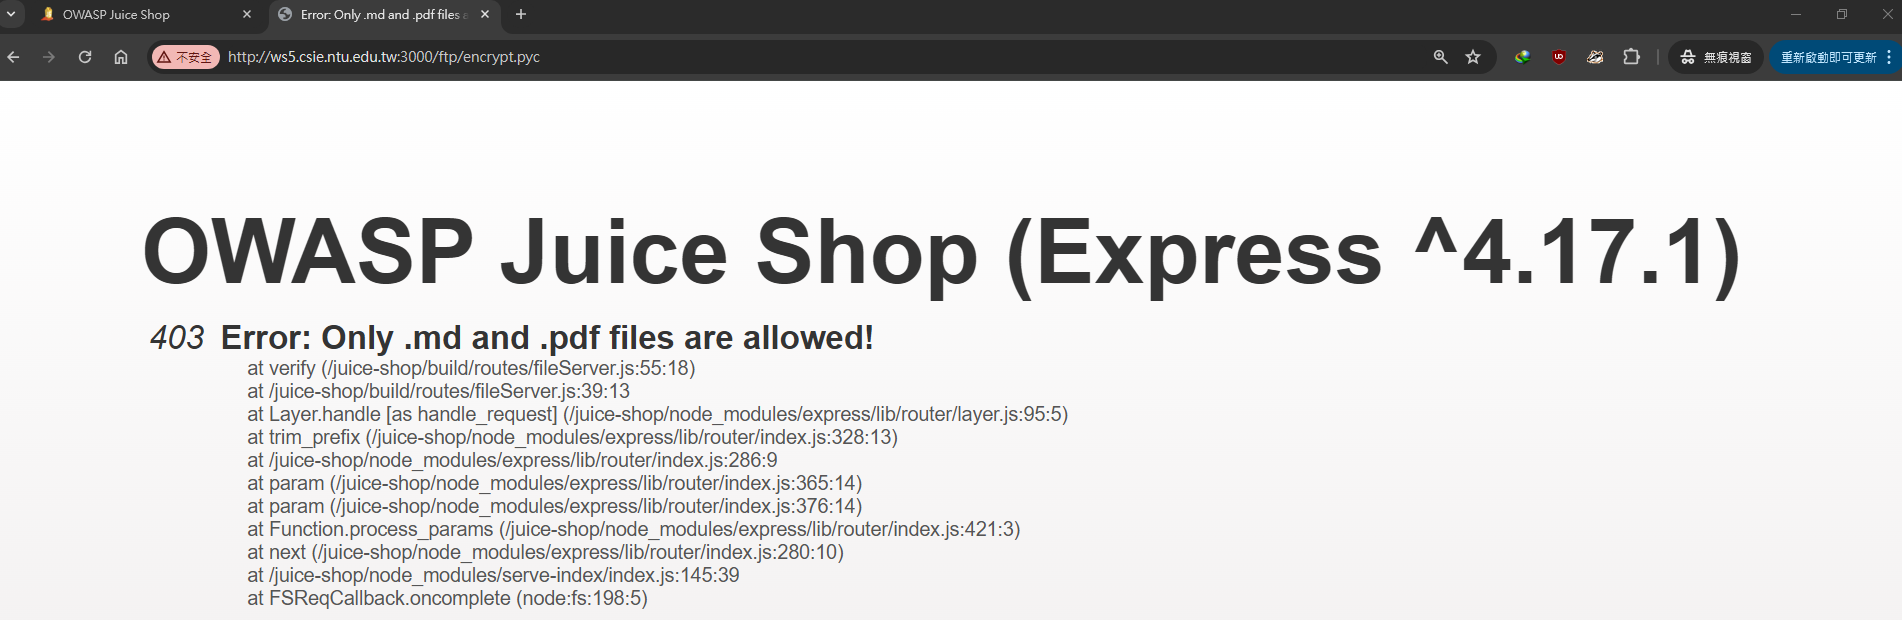
\includegraphics[width=\linewidth]{4-1-d_error.png}

    \textbf{Result}

    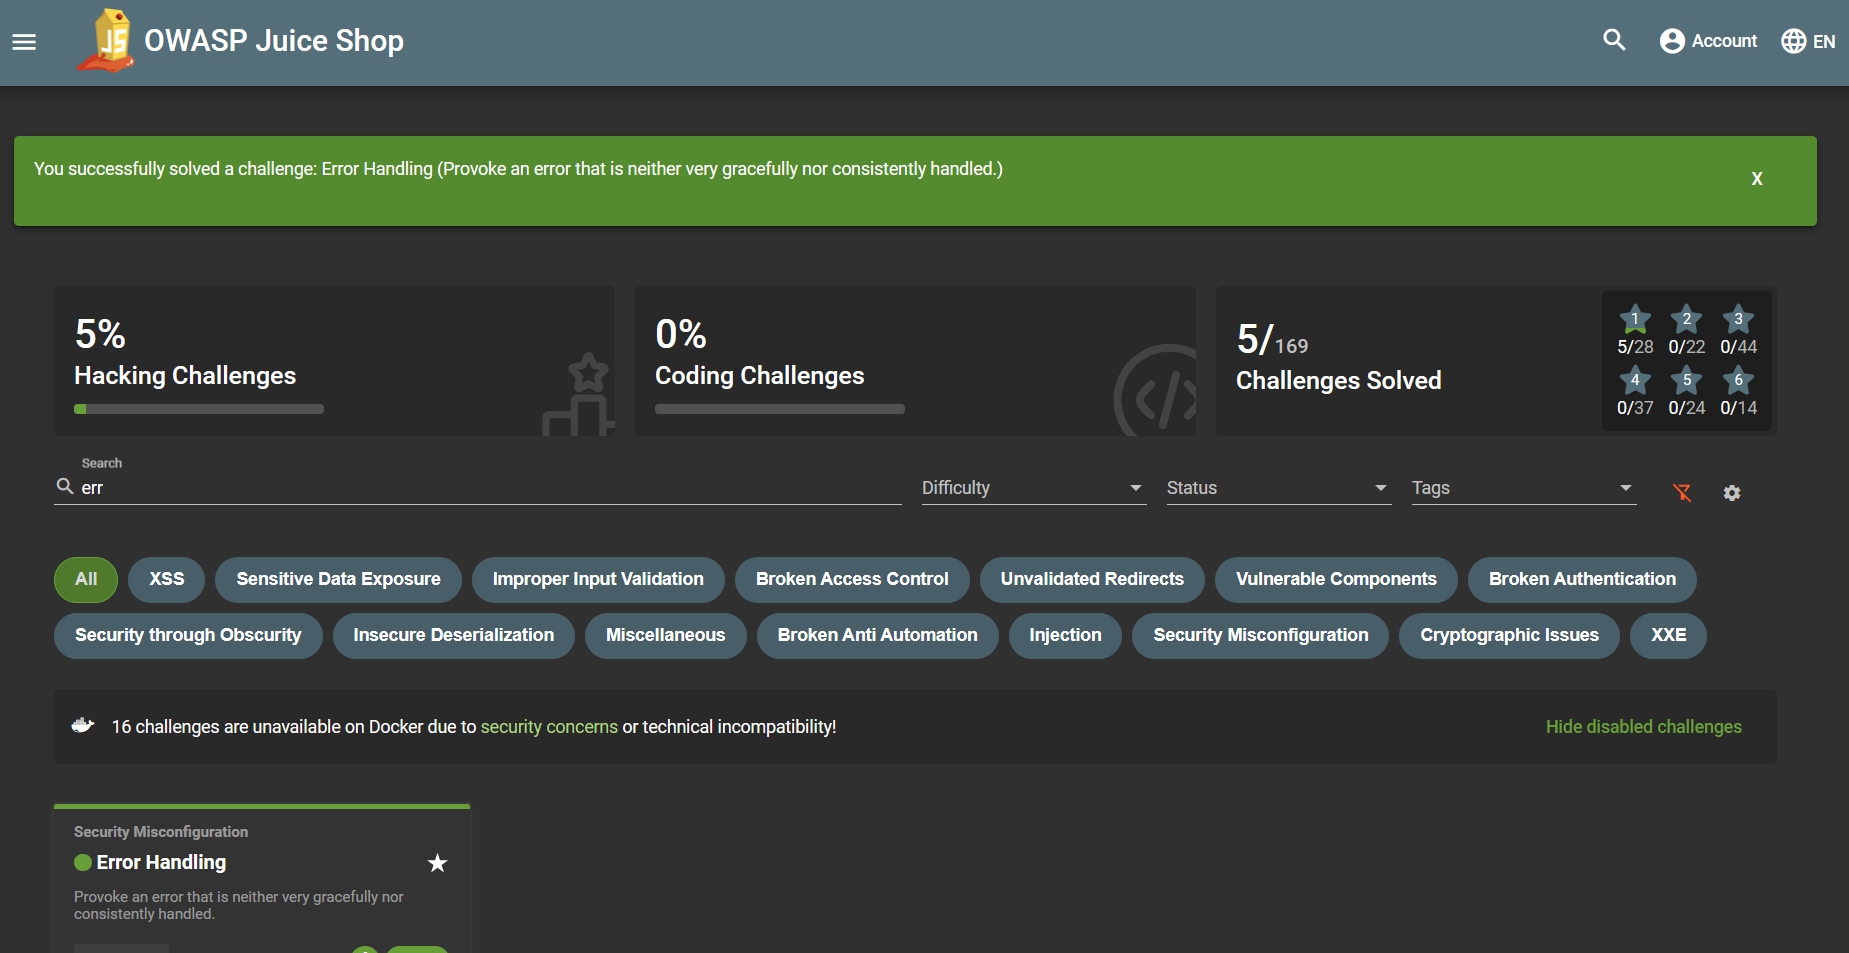
\includegraphics[width=\linewidth]{4-1-d_solved.png}

    \textbf{Explanation}

    When errors are not properly handled, it make leak information or
    configuration about the server, which is a potential weakness for
    attackers to exploit.

    To prevent this vulnerability, we have to configure the server to
    properly handle errors, and avoid displaying any debug information
    in a production environment.

    \textbf{References}
    \begin{itemize}
      \item \href{https://pwning.owasp-juice.shop/companion-guide/latest/part2/security-misconfiguration.html}{Security Misconfiguration :: Pwning OWASP Juice Shop}
    \end{itemize}

    \pagebreak
    \item \textbf{Login Admin}

    \textbf{Steps}
    \begin{enumerate}[label=(\roman*)]
      \item In the ``Login" (\verb|/#/login|) page, type \verb|'| as Email and
      a random string for the password.

      \item In Chrome DevTools, inspect the failed \verb|/rest/usr/login| request. The
      SQL command is in the response. This allows us to perform SQL injection.
      \begin{minted}[fontsize=\small, breaklines]{json}
{
  "error": {
    "message": "SQLITE_ERROR: unrecognized token: \"962012d09b8170d912f0669f6d7d9d07\"",
    // ...
    "sql": "SELECT * FROM Users WHERE email = ''' AND password = '962012d09b8170d912f0669f6d7d9d07' AND deletedAt IS NULL",
    "parameters": {}
  }
}
      \end{minted}
      \item Back to the login page, type \verb|' UNION SELECT * FROM Users --| as the email.
      We have successfully logged into the admin account.
    \end{enumerate}

    \textbf{Result}

    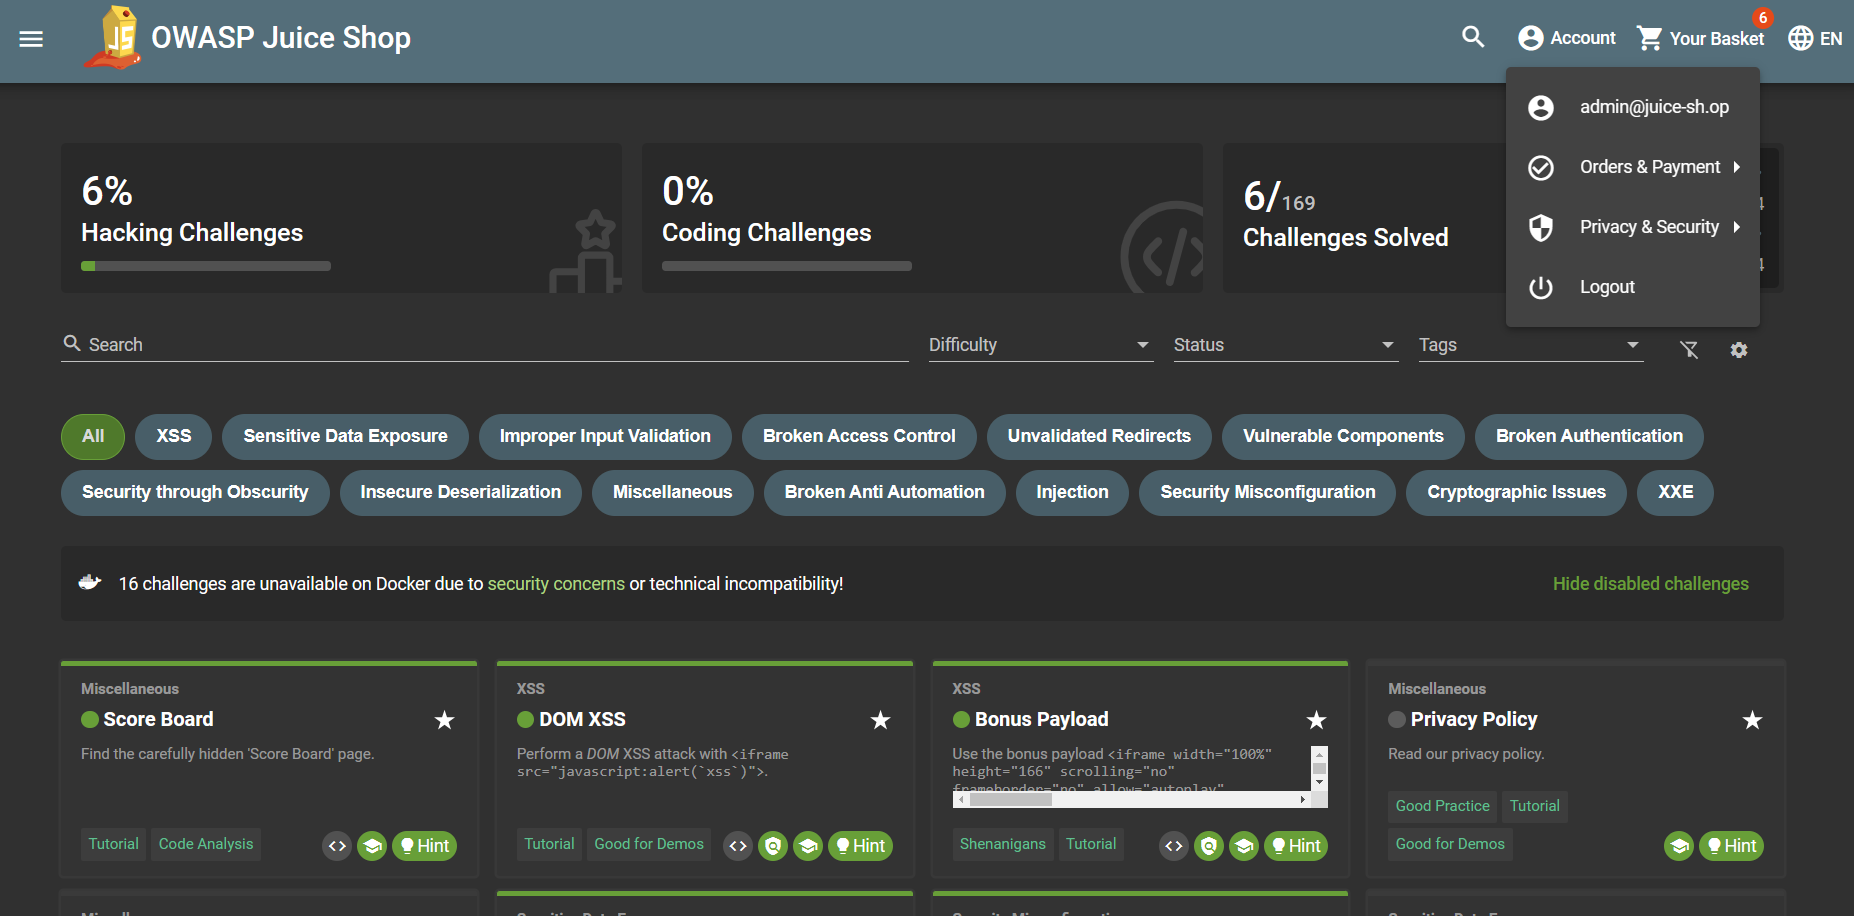
\includegraphics[width=\linewidth]{4-1-e_solved.png}

    \textbf{Explanation}

    This attack is possible because the SQL command is included in the response, and
    the HTML form allows us to input special characters used in SQL commands as the
    email.

    To prevent this type of attack, we never reveal SQL commands to the public, and
    enforce syntax checking for the email and password fields.

    \textbf{References}
    \begin{itemize}
      \item \href{https://portswigger.net/web-security/sql-injection/union-attacks}{SQL injection UNION attacks | Web Security Academy}
    \end{itemize}
  \end{enumerate}

  \pagebreak
  \subsection{CSRF}
  \textbf{Cross-site request forgery} (CSRF) refers to an attack
  where unauthorized commands are sent to a website as if they are
  from a trusted user of the website. This is usually done by the attacker
  tricking an innocent victim into submitting a maliciously crafted web request
  to a website that the user has access to. Because the victim's browser has the
  cookie or session keys, the forged request would be sent as the victim's
  identity, therefore exposing weaknesses.

  \textbf{References}
  \begin{itemize}
    \item \href{https://en.wikipedia.org/wiki/Cross-site_request_forgery}{Cross-site request forgery - Wikipedia}
    \item \href{https://developer.mozilla.org/en-US/docs/Glossary/CSRF}{CSRF - MDN Web Docs Glossary: Definitions of Web-related terms | MDN}
  \end{itemize}
\end{document}
